\subsubsection{Datafiles}
\label{sec:view_datafiles}

\paragraph{}
The datafile page is linked in the default navigation menu under the session tab. It comprises a div for information about the currently selected datafile(s) and a second div whose contents are AJAX generated when the 'View All Datafiles' button is clicked. The relationships between datafiles in ROME can be represented as a directed acyclic graph and GraphViz is used to generate an image of the datafiles, with edges marked with the name of the process which generated the child datafile. Placeholder datafiles, which are the yet-to-be-created results of queued jobs, have there names shown in red. Selected datafiles are shaded yellow. Each of the datafiles is clickable. Clicking a selected datafile will deselect it and clicking a deselected datafile will select it. A simple example is illustrated in figure \ref{fig:view_datafiles}

\begin{figure}[h]
\centering
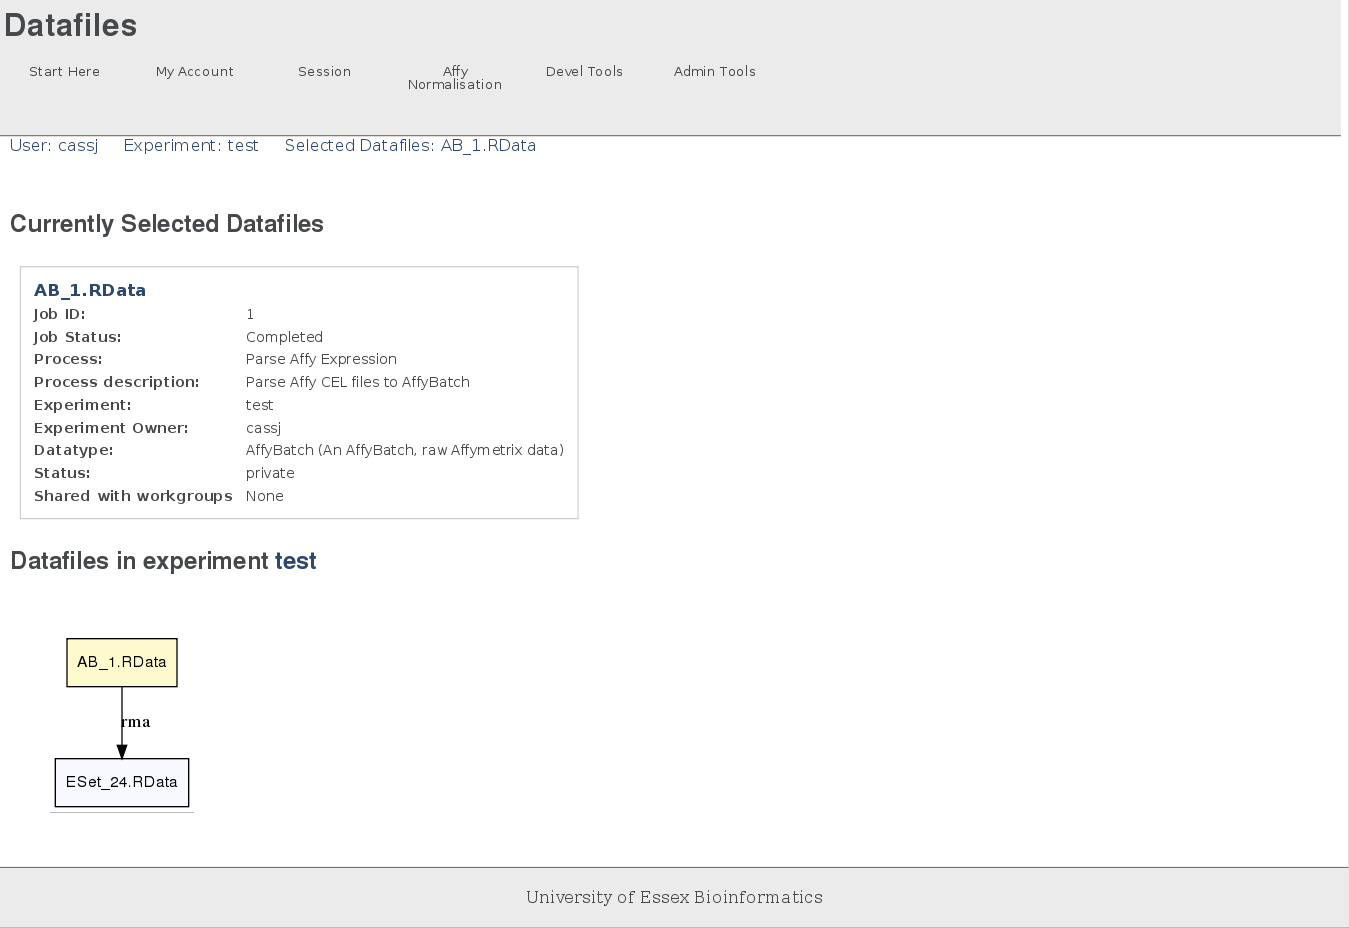
\includegraphics[scale=0.45, angle=90]{../rome/docs/images/screenshots/datafiles}
\caption{The Datafile Page}\label{fig:view_datafiles}
\end{figure}

\clearpage